% !TEX encoding = UTF-8 Unicode
\documentclass[a4paper]{article}

\usepackage{color}
\usepackage{url}
\usepackage[T2A]{fontenc} % enable Cyrillic fonts
\usepackage[utf8]{inputenc} % make weird characters work



\usepackage{graphicx}
\graphicspath{ {./slike/} }

\usepackage[english,serbian]{babel}
%\usepackage[english,serbianc]{babel} %ukljuciti babel sa ovim opcijama, umesto gornjim, ukoliko se koristi cirilica

\usepackage[unicode]{hyperref}
\hypersetup{colorlinks,citecolor=green,filecolor=green,linkcolor=blue,urlcolor=blue}

\usepackage{listings}

%\newtheorem{primer}{Пример}[section] %ćirilični primer
\newtheorem{primer}{Primer}[section]

\definecolor{mygreen}{rgb}{0,0.6,0}
\definecolor{mygray}{rgb}{0.5,0.5,0.5}
\definecolor{mymauve}{rgb}{0.58,0,0.82}

\lstset{ 
  backgroundcolor=\color{white},   % choose the background color; you must add \usepackage{color} or \usepackage{xcolor}; should come as last argument
  basicstyle=\scriptsize\ttfamily,        % the size of the fonts that are used for the code
  breakatwhitespace=false,         % sets if automatic breaks should only happen at whitespace
  breaklines=true,                 % sets automatic line breaking
  captionpos=b,                    % sets the caption-position to bottom
  commentstyle=\color{mygreen},    % comment style
  deletekeywords={...},            % if you want to delete keywords from the given language
  escapeinside={\%*}{*)},          % if you want to add LaTeX within your code
  extendedchars=true,              % lets you use non-ASCII characters; for 8-bits encodings only, does not work with UTF-8
  firstnumber=1000,                % start line enumeration with line 1000
  frame=single,	                   % adds a frame around the code
  keepspaces=true,                 % keeps spaces in text, useful for keeping indentation of code (possibly needs columns=flexible)
  keywordstyle=\color{blue},       % keyword style
  language=Python,                 % the language of the code
  morekeywords={*,...},            % if you want to add more keywords to the set
  numbers=left,                    % where to put the line-numbers; possible values are (none, left, right)
  numbersep=5pt,                   % how far the line-numbers are from the code
  numberstyle=\tiny\color{mygray}, % the style that is used for the line-numbers
  rulecolor=\color{black},         % if not set, the frame-color may be changed on line-breaks within not-black text (e.g. comments (green here))
  showspaces=false,                % show spaces everywhere adding particular underscores; it overrides 'showstringspaces'
  showstringspaces=false,          % underline spaces within strings only
  showtabs=false,                  % show tabs within strings adding particular underscores
  stepnumber=2,                    % the step between two line-numbers. If it's 1, each line will be numbered
  stringstyle=\color{mymauve},     % string literal style
  tabsize=2,	                   % sets default tabsize to 2 spaces
  title=\lstname                   % show the filename of files included with \lstinputlisting; also try caption instead of title
}




% Dodao Petar
\usepackage[]{algorithm2e}
\usepackage{subcaption}
%%%%%

\begin{document}

\title{Primene memetskog algoritma\\ \small{Seminarski rad u okviru kursa\\Metodologija stručnog i naučnog rada\\ Matematički fakultet}}

\author{Bogićević Marica, Karanović Boris, Košanin Petar, Šašić Filip\\ kontakt email prvog, boskonet@gmail.com, trećeg, četvrtog autora}

%\date{9.~april 2015.}

\maketitle

\abstract{
 Kroz ovaj rad čitalac će se upoznati sa memetskim algoritmom i njegovim primenama. Prikazan je postupak primene algoritma na dva NP problema: 
 \emph{problem bojenja grafa} i \emph{problem trgovačkog putnika}. Takođe je naveden i \emph{problem prepoznavanja zajednica} koji ilustruje i primenu memetskog algoritma na realan problem. Primene memetskog algoritma su dosta raznolike, što svrstava celu familiju evolutivnih algoritama kojoj i sam pripada, među popularnim temama u akademskim i industrijskim krugovima. 
}

\tableofcontents

\newpage

\section{Uvod}
\label{sec:uvod}

Memetski algoritam je prvi put uveden u računarstvo 1989. godine od strane Pabla Moscata \cite{towardsmemetic}. Predstavlja hibridizaciju tradicionalnog, populacionog, genetskog algoritma sa metodama lokalne pretrage kako bi umanjio verovatnoću prevremene konvergencije. Danas, memetski algoritmi su poznati i pod nazivima: $hibridni$ $evolutivni$ $algoritmi$ i $kulturalni$ $algoritmi$. U nastavku je dat prikaz memetskog algoritma u njegovoj osnovnoj formi.

\begin{figure}[h!]
    \centering
	\begin{subfigure}[normla]{0.3\textwidth}
		\hspace*{-1cm}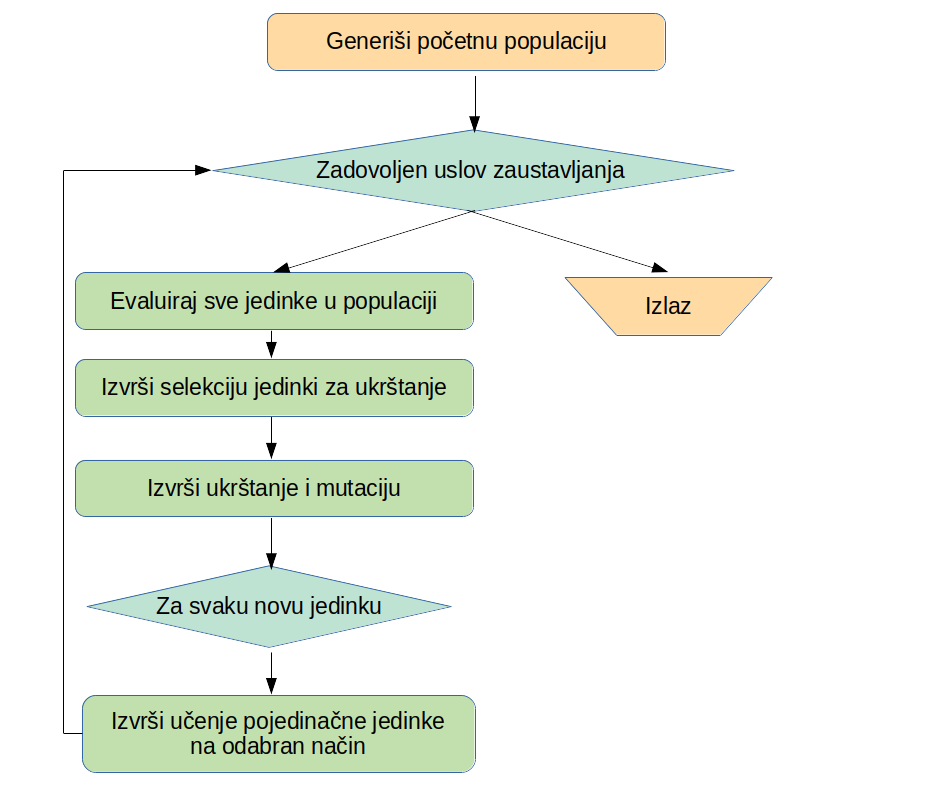
\includegraphics[scale=0.3]{slike/memeticdrawcrop.png}
		\caption{Memetski algoritam}
		\label{memeticdrawcrop}
	\end{subfigure}
\label{memeticdrawcrop.png}
\end{figure}

Prilikom dizajniranja samog memetskog algoritma, osim parametara koji su neophodni i za osnovni genetski algoritam, potrebno je odrediti još nekoliko parametara specifičnih za memetski algoritam. 

\begin{itemize}
  \item Koliko često trebamo vršiti poboljšanje pojedinačnih jedinki ?
  \item Na kojim jedinkama ćemo vršiti poboljšanje ?
  \item Koje metode ćemo koristiti za jedinke ?
  \item Koliko vremena ćemo potrošiti na poboljšanja ? 
\end{itemize}

Određivanje ovih parametara predstvavlja izazov prilikom kreiranja memetskog algoritma, i direktno utiču na njegovu efikasnost. 


\section{Primene memetskog algoritma}
\label{sec:primene_memetskog_algoritma}
Memetski algoritam nalazi uspešne primene u mnogim realnim problemima. Kao i genetski algoritam, može se koristiti i u rešavanju raznih NP-teških problema, poput problema trgovačkog putnika, minimalnog bojenja grafa, problem ranca i raznih drugih problema. 
Mnoge moderne primene podrazumevaju korišćenje memetskog algoritma u oblastima analize poslovanja biznisa, istraživanje podataka, prepoznavanje šablona, dizajniranja električnih kola, mašinskog učenja. Takođe, značajna je i primena u bioinformatici. 


\subsection{Problem bojenja grafa}
\label{sec:bojenje_grafa}
Neka je zadat neusmeren graf $G = (V, E)$, gde je $V$ skup čvorova, a $E$ skup grana tog grafa. 
Bojenje grafa $G$ predstavlja problem dodeljivanja $''$boja$''$ elementima grafa\footnote{Problem isključivo zavisi od \textit{broja} boja, a ne od konkretnih boja.}. 
Bojenje čvorova je pridruživanje po jedne boje svakom čvoru grafa $G$. 
Dodavanjem ograničenja maksimalnog broja boja, dobijamo problem k-bojenja grafa. \textit{Ispravno k-bojenje grafa} $G$ je ono za koje ne postoje dva susedna čvora\footnote{Dva čvora su susedna, ako postoji grana koja ih povezuje.} koji su obojeni istom bojom. 
Drugim rečima, ispravno k-bojenje grafa deli čvorove skupa $V$ u $k$ nezavisnih podskupova, pri čemu jedan taj podskup čine nesusedni čvorovi, obojeni istom bojom. Na slici \ref{bojene_grafa} prikazan je primer ispravnog bojenja grafa.


\begin{figure}[h!]
	\centering

	\begin{subfigure}[normla]{0.3\textwidth}
		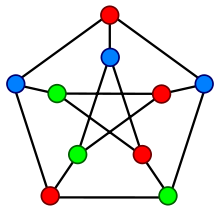
\includegraphics[scale=0.3]{bojene_grafa1}
		\caption{Primer ispravnog bojenja čvorova grafa}
		\label{bojenje_grafa1}
	\end{subfigure}
	~
	\begin{subfigure}[normla]{0.3\textwidth}
		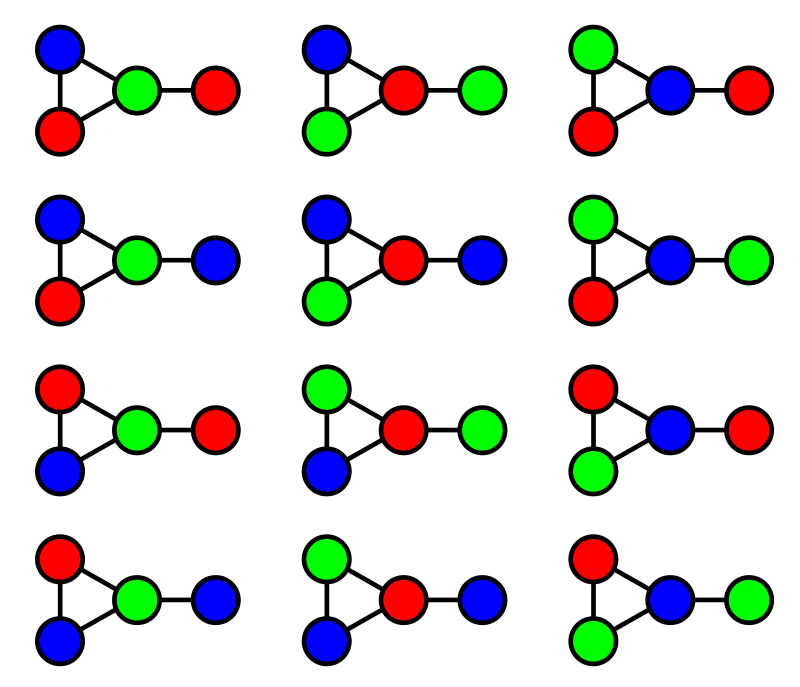
\includegraphics[scale=0.1]{bojenje_grafa2}
		\caption{Različita ispravna bojenja čvorova grafa}
		\label{bojenje_grafa2}
	\end{subfigure}
		\caption{Slika (a) prikazuje ispravno 3-bojenje Pitersonovog grafa, dok na slici (b) prikazano je 12 različitih načina 3-bojanja grafa. Izvor slika \cite{graph_coloring} }
\label{bojene_grafa}
\end{figure}

Pored svoje teoretske značajnosti kao NP-kompletan problem \cite{zivkovic_algoritmi}, bojenje grafa nalazi primenu u praksi, a neki od problema koji se svode na bojenje grafa su alokacija registara, izrada rasporeda, raspoređivanje komunikacije satelita \cite{lu2010memetic}.

Rešavanje problema bojenja grafa može se predstaviti preko rešavanja serije problema k-bojenja grafa \cite{galinier1999hybrid}. 
Naime, rešavanje problema počinje sa inicijalnom vrednošću $k \leq |V|$. 
Ako se nađe rešenje za $k$, vrednost $k$ postavljamo na $k-1$, i ponavljamo proces sve dok ne naiđemo na $k$ za koje ne postoji rešenje.

U nastavku biće opisane tri varijacije memetskog algoritma za rešavanje problema bojenja grafa. 

\subsubsection{HCA}
U radu \cite{galinier1999hybrid}, predložen je HCA(eng. Hybrid Coloring Algorithm) za rešavanje problema bojenja grafa.
HCA čine 4 glavne komponente, \textit{generator inicijalne populacije}, \textit{operator ukrštanja}, \textit{lokalna pretraga}, i \textit{pravila ažuriranja populacije}.

Jednu jedinku populacije čini podela skupa $V$ na $k$  disjunktnih podskupova $\{V_1, V_2, ...., V_k\}$. Takođe, dodaju se penali onim jedinkama koje sadrže susedne čvorove. Inicijalnu populaciju mogu činiti jedinke koje predstavljaju nedopustiva rešenja\footnote{Rešenje je nedopustivo ako ne zadovoljava nametnuta ograničenja problema.}. 
Lokalna pretraga se zatim koristi za unapređivanje svake jedinke, i eventualno ispravljanje nedopustivih rešenja.
HCA za lokalnu pretragu koristi tabu pretragu \cite{tabu_pretraga_miskovic}.
Operator ukrštanja konstruiše nova k-bojenja i zatim koristi lokalnu pretragu radi daljeg unapređivanja novih jedinki. 
Korišćen operator ukrštanja od strane HCA je GPX(eng. Greedy Partition Crossover\cite{galinier1999hybrid}.
Konačno, pravilo ažuriranja populacije bira jedinke koje prelaze u novu generaciju, a koje će biti zamenjene.
\subsubsection{MACOL}
MACOL \cite{lu2010memetic} predstavlja još jednu verziju memetskog algoritma za rešavanje problema bojenja grafa. Za inicijalizaciju populacije, MACOL koristi randomizovanu verziju DANGER \cite{glover1996coloring} metode. 
Za razliku od HCA pristupa, MACOL predlaže novu metodu ukrštanja AMPaX(eng. Adaptive Multi-Parent crossover) \cite{lu2010memetic}, koju autori opisuju kao proširenu verziju GPX metode. Jedna od razlika je u tome što u ukrštanju učestvuje dve ili više jedinki. Slično kao i u HCA pristupu, MACOL koristi tabu pretragu.

\subsubsection{HEAD}
HCA (ili drugačije Hybrid Evolutionary Algorithm(HEA)) je do 2012. godine davao najbolje rezultate nad DIMACS \cite{10.5555/548182} grafovima. HEAD (eng. Hybrid Evolutionary Algorithm in Duet) \cite{moalic2018variations} predstavlja unapređenje HCA algoritma. Osnovno svojstvo HEAD algoritma je veličina populacije, tj populaciju čine \textit{dve} jedinke. Nakon nasumične inicijalizacije jedinki, vrši se ukrštanje korišćenjem GPX metode. Zatim, HEAD koristi tabu pretragu kako bi unapredio jedinke, i konačno se vrši izbor jedinki koje će činiti sledeću generaciju. 

Kako populaciju čine samo dve jedinke, veliki problem HEAD algoritma je prevremena konvergencija. Da bi se zaobišao navedeni problem, HEAD uvodi novo pravilo ažuriranja populacije, tj, koriste se dve pomoćne jedinke $elita_1$ i $elita_2$.

\begin{figure}[h!]
\centering
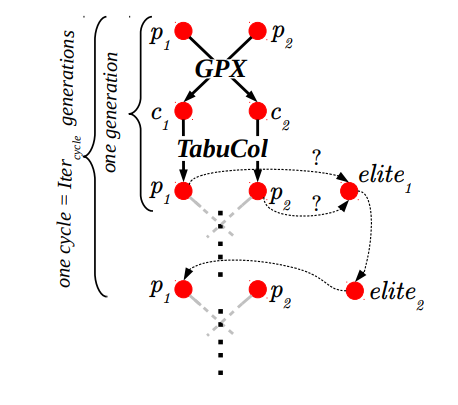
\includegraphics[scale=0.5]{head_algoritam}
\caption{Dijagram HEAD algoritma}
\label{head_algoritam}
\end{figure}

Naime, $elita_1$ predstavlja najbolje rešenje trentutne generacije, dok $elita_2$ najbolje rešenje prethodne. U svakoj iteraciji algoritma, jedna od novonastalih jedinki ukrštanjem zamenjuje se sa $elita_2$ jedinkom \ref{head_algoritam}. Pretpostavka je da $elita_2$ se dovoljno razlikuje od jedinki trenutne generacije, i samim tim da doprinosi diverzifikaciji populacije. Dijagram ažuriranja populacije HEAD algoritma prikazan je na slici \ref{head_algoritam}.




\subsection{Problem trgovačkog putnika}
\label{sec:trgovacki_putnik}

Problem trgovačkog putnika(eng. Travelling Salesman Problem - TSP) je klasičan problem u polju diskretne i kombinatorne optimizacije. Spada u grupu NP-teških problema čija je složenost O(n!). Matematičke probleme slične njemu prvi je razmatrao Euler koji se bavio pitanjem kako će skakač na šahovskoj tabli posetiti sva 64 mesta samo jednom. Početkom dvadesetog veka matematičar William Rowan Hamilton i Thomas Kirkman su razmatrali probleme koji se svode na problem trgovačkog putnika. 


Opšta forma problema TSP je javlja tridesetih godina dvadesetog veka, a pojam $"$trgovački putnik$"$ prvi put je upotrebljen 1932 godine od strane Karla Mengera koji je u svom radu spomenuo brute-force algoritam i definisao TSP onako kako ga danas poznajemo. Problem je vremenom postajao sve više popularan i izučavan od strane mnogih naučnika.

Neformalna formulacija problema: Dato je n gradova i poznate su sve udaljenosti između njih. Trgovački putnik treba da obiđe sve gradove i da se na kraju vrati u grad odakle je krenuo, ali da pri tome razdaljina koju pređe bude najkraća.

\subsubsection{Prethodni radovi}
\label{subsec:prethodniRadovi}

MTSP (Minimalni problem trgovačkog putnika) je jedan najproučavanijih kombinatorno optimizacionih problema. 

U \cite{Handbook} je prikazan kratak pregled početnih Memetskih algoritama(MA) za TSP i predstavljali su približna optimalna rešenja za mali broj gradova. Iako rezultati nisu bili konačni, bili su ohrabrujući i naredna primena Memetskih algoritama na TSP (i na druge NP-Optimizacione probleme) je bila inspirisana tim ranijim radovima.


U \cite{Memetic}, MA su korišćeni sa nekoliko nestandardnih karakteristika. U \cite{Memetic}, lokalna pretraga je bazirana na moćnoj Navođenoj lokalnoj pretrazi (GLS), Voudorisovoj i Tsangovoj metaheuristici. Ovaj algoritam je poređen sa Lokalnom pretragom sa više početaka (MSLS), Navođenom lokalnom pretragom i sa Memetskim algoritmom. Lokalna pretraga kod MA je bila ista kao i kod GLS-a, ali bez navođenja. U našem eksperimentu smo koristili instance preuzete sa TSPLIB\cite{TSPLIB}. Ni u jednom slučaju MLSL nije mogao da pronadje optimalnu turu, dok su ostala tri pristupa mogla da je pronađu. Od 31 testirane instance, MA je rešio optimalnih 24, MLSL 0, MA sa jednostavnom lokalnom pretragom 10 i GLSL 16. 

Merz i Freisleben u \cite{ASIM} pokazuju različite kombinacije lokalne pretrage i genetske pretrage za TSP(i asimetričnu verziju ATSP) i pokazuju specifičnu ulogu ukrštanja i mutacije. U njihovom pristupu, inicijalna populacija je skup lokalnih optimuma po Lin-Kernighan heuristici, koji je osnova za GA sa skoro optimalnim rešenjima pri inicijalizaciji. Važna stavka njihovog pristupa je da selekcija nije $(\mu +\lambda)$, ni $(\mu,\lambda)$ već mešavina ta dva. 

Markov Chains i iterativni Lin-Kernighan tehnike su specijalni slučajevi tehnike Merz-a i Freisleben-a. Njihova mutacija i selekcija je tradicionalnija. Važno je naglasiti da je Memetski algoritam Merz-a i Freisleben-a možda najuspešnija metaheuristika za TSP i ATSP  a prethodno opisane šeme su bile pobednički algoritam na Prvom internacionalnom takmičenju u evolutivnoj optimizaciji.

\subsubsection{Metodološki pristup}
\label{subsec:metodologija}

U nastavku ćemo opisati našu metodologiju i MA za TSP. Naša svrha je da prikažemo potencijal pretrage i različitost našeg pristupa. Nama nije cilj da napravimo specijalizovani TSP rešavač. Mi smo koristili naivne i generičke genetske operatore (ukrštanje i mutacija). Lokalna pretraga ne koristi nikakvo znanje o instanci koja je rešena osim onih koje su obezbedile fitnes funkcije. Na ovaj način možemo da garantujemo da će svaki pronađeni benefit biti svojstvo pristupa, a ne posledica korišćenja moćnih operatora. U svim prethodno navedenim Memetskim algoritmima za TSP, inteligentni operatori su korišćeni u formi specijano dizajnirane mutacije, ukrštanja i lokalne pretrage. Štaviše, lokalna pretraga je korišćena u navedenim radovima koristeći znanje o instancama (to jest listu najbližih suseda, kd-drveta...). Osim toga,ne postoji nigde u literaturi nešto poput $"$standardnog$"$ MA za TSP s kojim bismo mogli da pravimo poređenje.


\subsubsection{Memetski algoritam primenjen na problem trgovačkog putnika }
\label{subsec:MATSP}

U ovom odeljku ćemo opisati novu prilagođavajuću šemu. Pokazaćemo kako nelinearna interakcija između osnovnog genetskog algoritma i lokalne pretrage/diverzifikovani proces (koja je regulisana posmatranjem populacije genetskih algoritama) daje poboljšanje u metaheuristici globalne pretrage.

\subsubsection{Opis Memetskog algoritma }
\label{subsec:MA}

Korišćeni pseudokod MA je: \\

\textbf{Begin} \\
1\hspace{0.5cm}{\textit{Initialize population Parents;} \\
2\hspace{0.5cm}\textbf{Repeat Until} }\textit{(Finalization\_criteria\_met)} \textbf{Do} \\
3\hspace{1cm} \textit{Local\_Search(Parents,Pls); }\\
4\hspace{1cm} \textit{mating\_pool := Select\_mating(Parents);} \\
5\hspace{1cm} \textit{Offspring s:= Cross(mating\_pool);} \\
6\hspace{1cm} \textit{Mutate(Offsprings);} \\
7\hspace{1cm} \textit{Parents := Select(Parents,Offsprings);} 

\textbf{End.} \\

U ovoj osnovnoj šemi, Select(...) je $(\mu + \lambda)$ ili $(\mu,\lambda)$ strategije, predstavljajući dva ekstrema selektivnog pritiska, sa +$\setminus$- strategijom imajući najveći pritisak i - najnižu strategiju. Select\textunderscore mating(...) je turnirska selekcija. U slučaju +$\setminus$- strategije, data jedinka može biti modifikovana više puta tokom svog $"$života$"$ od strane lokalne pretrage ili mutacije zato što nam strategija dopušta da jedinka opstaje. Najbolja jedinka se nikada ne modifikuje lokalnom pretragom, tako da u funkciji lokalne pretrage pozivamo funkciju Apply\_Move(indip):\\


\textbf{Begin} \\
1\hspace{0.5cm}  \textit{ /* This is a minimizing process */ } \\
2\hspace{0.5cm} \textit{{ prevFitness = fitness(indip);}} \\
3\hspace{0.5cm}\textit{ Modify(indip);}  \\
4\hspace{0.5cm} \textit{nFitness = fitness(indip);} \\
5 \hspace{0.5cm}\textbf{If}\textit{(prevFitness > nFitness)} \textbf{Then} \\
6  \hspace{1cm} \textit{Accept configuration}; \\
7 \hspace{0.5cm}\textbf{Else} \\
8\hspace{1cm}\textit{  deltaE=nFitness-prevFitness;} \\
9 \hspace{1cm} \textit{ treshold = $e^{-k*\frac{deltaE}{temperature}}$} \\
10 \hspace{1cm} \textbf{If}\textit{(random(0,1)<treshold)} \textbf{Then} \\
11\hspace{1.5cm} \textit{ Accept configuration;} \\
12 \hspace{1.5cm}   \textit{/* even if worse than the previous one */ } \\
13 \hspace{1cm} \textbf{ Else} \\
14 \hspace{1.5cm}  \textit{ Reject changes;} 

\textbf{End.} \\


Mora biti naznačeno da Modify(...) može biti bilo koji potez lokalne pretrage (to jest 2swap, ubacivanje gradova...). Samoadaptacija lokalne pretrage eksploracijskom ili eksplatacijijskom ponašanju je regulisana parametrom temperature. U slučaju predstavljenom iznad, cela populacija deli istu temperaturu. Ta temperatura određuje stepen kojim će kretanje uzbrdo biti dozvoljeno. Pošto je temperatura inverzno proporcionalna širenju fitnesa u populaciji, fitnes konvergira dok temperatura raste. Posledica ovoga je da će svaka jedinka u populaciji biti više $"$nervozna$"$ i pokušaće da se udalji od inicijalne pozicije, istražujući prostor pretrage. U nekom trenutku fitnes će se širiti, spuštajući temperaturu populacije. Mi obezbeđujemo modifikaciju najboljih jedinki lokalnom pretragom, stoga je uslov najboljeg fitnesa održan.  

\subsubsection{Primena memetskog algoritma na TSP}
\label{subsec:primena}

Primenili smo MA(...), Localsearch(...) i ApplyMove(...) na TSP sa modifikacijom definicije temperature koja je bila postavljena na 

$\frac{1}{|maxFitness - averageFitness|}$ da bi bila bolja dinamičnost. Modify(...) procedura je koristila two\_swap (TS) pomeranje. TS selektuje podturu i invertuje gradove. To dovodi do 4 promene putanje u datoj turi. Nazvana je two\_swap zato što pravi dve promene putanja u originalnoj turi zarad dve nove putanje. Modify(...) bira random broj (između 1 i 10\% od instancne veličine) koji određuje koliko vezanih primena two\_swap(...) će biti primenjeno na jedinku. Posle primene pomeraja, nova jedinka će biti prihvaćena na osnovu Boltzmann-ove distribucije bazirane na temperaturi trenutne populacije. 

Slede detalji MA:
Koristili smo populaciju od 50 jedinki. Ukrštanje, mutacija i lokalna pretraga su  primenjeni sa verovatnoćom od 0.8, 0.05 i 1.0 redom. Ove verovatnoće su bile fiksne sve vreme. Nije rađena iscrpna optimizacija parametara, već su određivani empirijski zavisno od broja pokretanja. Vrednost k je 0.01 u $(\mu,\lambda)$ strategiji, a 0.001 u $(\mu + \lambda)$. Svaka jedinka radi lokalnu pretragu/diverzifikovanu fazu u svakoj generaciji, osim najboljih jedinki. Selekcija je Turnirska veličine 2. GA je u jednom slučaju mirnog stanja sa (50 + 50) selekcionom strategijom, a u drugom slučaju (50,50) selektivne strategije je bilo korišćeno. Za kodiranje smo koristili niz intidžera koji imaju sledeće značenje: ako pozicija i ima intidžer j, onda putanja povezuje gradove i i j, (i,j) postoji u turi. Ukrštanje prihvata dva roditelja i generiše potomke počevši od random grada. Daje detetu najkraću putanju od bilo kojeg roditelja. Ako ni jedna putanja od oba roditelja nije slobodna, onda se dodaje random putanja. Mutacija je primena two\_swap operatora. Inicijalizacija populacije je random. 


\subsubsection{Eksperimentalne metode i rezultati}
\label{sec:rez}

U ovom delu ćemo predstaviti korišćene metode i dobijene rezultate. 
Kao što smo ranije spomenuli, koristimo instance iz baze TSPLIB \cite{TSPLIB} koja ima 76 gradova. Pokrenuli smo 30 simulacija za dve različite selektivne strategije, (50,50) i (50+50). Probali smo ova dva scenarija jer smo hteli da istražimo ne samo krajnju dužinu ture već i raznolikost populacije. Hteli smo da vidimo kako se ponaša naš samoadaptivni algoritam u ovim ekstremima. Testirali smo naš algoritam sa četiri druga algoritma: Standardni GA, Memetski algoritam za penjanje uz brdo (HC), Boltzmann-ov memetski algoritam za penjanje uz brdo, Memetski algoritam linearnog žarenja (LMA) i Samoadaptivni memetski algoritam (MA).


\begin{primer}U tabeli \ref{tab:tabela2} je prikazan kratak pregled statističke analize za dužinu ture ispod (50,50), strategija: + predstavlja algoritam čije ime u koloni postiže veću turu od imena u vrsti, - predstavlja algoritam čije ime u vrsti postiže manju turu od imena u koloni, a - ili + sa * predstavlja p-vrednost $\geq$ 0.01


\begin{table}[h!]
\begin{center}
\caption{Poređenje algoritama}
\begin{tabular}{||c|c|c|c|c|c||} \hline
Algorithms & GA& HC& BHC& LMA& MA\\ \hline
GA &  & - & + & + & +* \\ \hline
HC & + &  & + & + & +* \\ \hline
BHC & - & - &  & + & +* \\ \hline
LMA & - & - & - &  & +* \\ \hline
MA & -* & -* & -* & -* & \\ \hline
\end{tabular}
\label{tab:tabela2}
\end{center}
\end{table}

\end{primer}
















\subsection{Problem prepoznavanja zajednica}
\label{sec:prepoznavanje_zajednica}

TODO












\section{Zaključak}
\label{sec:zakljucak}

Svi algoritmi koji pripadaju evolutivnim algoritmima pretražuju prostor rešenja uz pomoć heuristika. Memetski algoritam za razliku od većine ostalih algoritama poseduje dosta veći broj parametara koji mu služe za navođenje kroz prostor rešenja. Upravo na tom mestu se dolazi i do problema. Pogrešnim izborom možemo dosta sporije doći do rezultata, kao i da dobijemo rešenje koje nije blizu optimalnog. Takođe, dobrim izborom parametara, memetski algoritam se pokazuje dosta efikasnijim od standardnog genetskog algoritma.

\addcontentsline{toc}{section}{Literatura}
\appendix
\bibliography{seminarski} 
\bibliographystyle{plain}

\appendix
\section{Dodatak}
TODO


\end{document}
